% !TeX spellcheck = cs_CZ
\begin{example}\label{AES:exam003}
  Na obr. \ref{enz:fig_pwm_gen} je realizován generátor šířkově modulovaného signálu pro
  simulátor \texttt{LTSpice}, jenž s výhodou využívá komponenty \texttt{B-source}, umožňující
  behaviorální popis požadovaného průběhu.

   {\centering
    \captionsetup{type=figure} 
    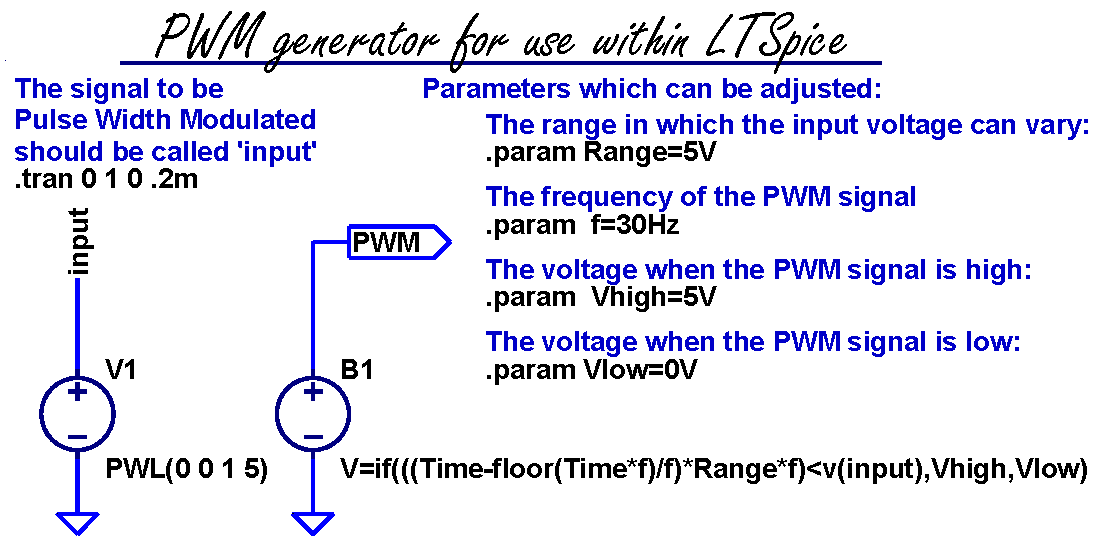
\includegraphics[width=0.8\linewidth]{LTspice_pwm_gen.pdf}
    \captionof{figure}{Realizace PWM generátoru pomocí komponenty B-source \emph{(Arbitrary 
               behavioral voltage or current source)} v LTSpice (soubor \texttt{pwm.asc})}
    \label{enz:fig_pwm_gen}
  \par}
  Podrobnějším pohledem na zápis rovnic dle obr. \ref{enz:fig_pwm_gen}, lze dojít k závěru, že
  zdroj \texttt{B1} na svůj výstup vnutí hodnotu parametru \texttt{Vhigh}, nebo \texttt{Vlow},
  podle výsledku rozhodovací funkce \texttt{if}. Tj. jeli \texttt{Time-floor(Time*f)/f)*Range*f)} 
  větší než \texttt{V(input)}, bude na výstupu $V_{high}= \SI{5}{\volt}$, v opačném případě 
  $V_{low} = 0V$. Funkce \texttt{floor} zaokrouhluje hodnotu svého argumentu na celé číslo 
  (\texttt{integer}), což vede na schodovitý průběh a funkce \texttt{Time} umožňuje do vztahu vnést 
  okamžitou hodnotu simulačního času. Vzájemný odečtením získáme pilový průběh, kterým se komparuje 
  s okamžitou hodnotou zdroje \texttt{V(input)}.

    {\centering
     \captionsetup{type=figure} 
     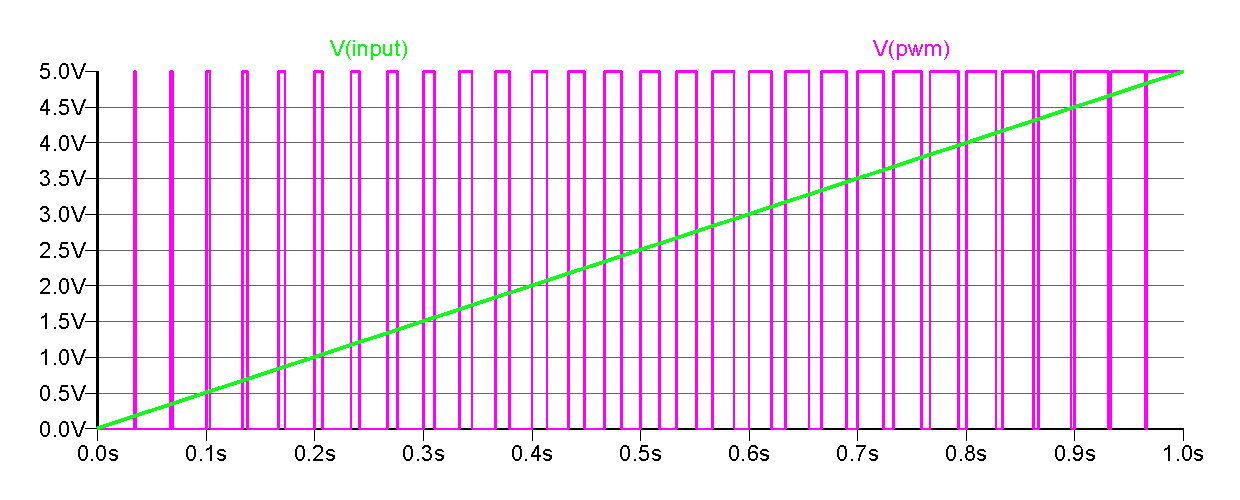
\includegraphics[width=1\linewidth]{LTspice_pwm_wave.pdf}
     \captionof{figure}{Výstupní signál \texttt{V(pwm)} z PWM generátoru na obr. 
                \ref{enz:fig_pwm_gen}  má-li rozhodovací napětí \texttt{V(in)} lineární charakter}
     \label{enz:fig_pwm_wave}
   \par}       
\end{example} 